\documentclass[a4paper,11pt]{article}
\usepackage{libertine}
\usepackage{inconsolata}
\usepackage{xcolor}
\usepackage[utf8]{inputenc}
\usepackage[T1]{fontenc}
\usepackage[english]{babel}
\usepackage[a4paper, left=1in, right=1in]{geometry}
\usepackage{calc}

\usepackage{mathpartir}
\usepackage{amsmath}
\DeclareMathOperator{\reft}{\textsf{ref}}
\DeclareMathOperator{\refnullt}{\textsf{ref null}}

\usepackage{tikz}
\usepackage{wrapfig}

\usepackage[backend=bibtex]{biblatex}
\addbibresource{report/report.bib}
\author{Aghilas Y. Boussaa \texttt{<aghilas.boussaa@ens.fr>}}

\title{\textsf{watib}: An optimising toolchain for modern WebAssembly}
\begin{document}
\maketitle
\begin{abstract}
  WebAssembly (Wasm) is a code format aiming at providing efficient execution.
  It now offers the features needed to be a compilation target for functional
  programming languages such as Scheme. Such a backend has been developped in
  the Bigloo compiler, relying on an external toolchain.

  We present \textsf{watib}, a WebAssembly Toolchain written In Bigloo. It has
  been integrated in the Bigloo Scheme compiler and is available as a standalone
  tool. We present \textsf{watib}'s architecture and compare our toolchain with
  the one used before.
\end{abstract}

\section{Introduction}
In 2024, a Wasm backend was added to the Bigloo~\cite{Bigloo} Scheme compiler.
It generated textual Wasm and relied on an external tool for the assembly.
\textsf{Watib} was developped as a replacement for this tool and has been
directly integrated in the Bigloo compiler. It is also available as a standalone
tool with a command-line
interface\footnote{\url{https://www.normalesup.org/~boussaa/watib/}}.

The rest of this section gives a high-level overview of WebAssembly and
\textsf{watib}. Section~\ref{val} details \textsf{watib}'s typechecker.
Section~\ref{opt} describes the design of the different optimisation passes and
the overall design of the optimiser. Section~\ref{bench} compares
\textsf{watib}'s and existing tools' performances We omit the assembly phase as,
once we have an intermediate representation, it is a straightforward
transcription of the specification.
\subsection{WebAssembly}
WebAssembly~\cite{haas2017bringing} is an assembly-like language for a
stack-based virtual machine. It aims at providing a fast, safe and portable
language endowed with a portable and efficient representation. New compilers
targetting Wasm are developped~\cite{emscripten, kotlin, ocaml}.

The WebAssembly standard~\cite{WebAssemblyCoreSpecification3} specifies typing
rules (validation), semantics, an abstract syntax and two concrete syntaxes
(formats) for the language. The binary format represents WebAssembly modules as
a sequence of bytes. It is taken as input by Wasm virtual machines such as
V8~\cite{V8} or SpiderMonkey~\cite{SpiderMonkey} and manipulated by toolchains
such as binaryen~\cite{Binaryen} or wasm-tools~\cite{WasmTools}. The textual
format represents WebAssembly modules as S-expressions. It is taken as input by
toolchains or written by humans (and compilers such as Bigloo).

The third version of the standard the standard adds features facilitating
compiling from functional languages. For instance, Wasm has now a garbage
collector, instructions for tail-calls (they are needed because the language
doesn't support goto) and exceptions. This version is still in draft, but the
mentionned features are stable and already implemented by the major Wasm
engines. Bigloo's Wasm backend relies on these features. They are demonstrated
in the example of Figure~\ref{ex}. For a more detailed introduction to
WebAssembly, see~\cite[Section~2.1]{phipps2023continuing}.

\begin{figure}[h]
  \begin{minipage}{\widthof{(type \$pair (sub \$pair-nil (struct (field \$cdr (ref \$pair-nil))}}
\begin{verbatim}
(type $pair-nil (sub (struct)))
(type $pair (sub $pair-nil (struct (field $cdr (ref $pair-nil))
                                   (field $car i32))))
(func $find-zero
  (param $l (ref $pair-nil))
  (result i32)
  (if (ref.test (ref $pair) (local.get $l))
    (then
      (if (i32.eqz (struct.get $pair $car
                     (ref.cast (ref $pair) (local.get $l))))
        (then (return (i32.const 1)))
        (else
          (return_call $find-zero
            (struct.get $pair $cdr
              (ref.cast (ref $pair) (local.get $l)))))))
    (else (return (i32.const 0))))
  (unreachable))
\end{verbatim}
  \end{minipage}

  \caption{A Wasm function testing if a list of integers contains 0}\label{ex}
\end{figure}

\subsection{Watib}
\textsf{Watib} handles type checking (the \texttt{Val} folder of the sources),
optimisation (the \texttt{Opt} folder) and assembly (the \texttt{Asm} folder) of
Wasm programs given in textual format\footnote{binary format support as input is
planned}. Function validation and optimisation is parallelisable. We added the
option to run them in an arbitrary number of threads using the \textsf{pthreads}
library. This feature, and thus the dependency on an external library is
optional which is requiered for integration with the Bigloo compiler.

The WebAssembly platform is in constant evolution. Features are added to the
engines before they are standardised. Thus potential users might want to be able
to use them as soon as possible. Long-term maintenance is one of our goals.
\textsf{Watib} has been designed to be able to keep up with the additions made
to the language. Adding a instruction that isn't a block can be done by putting
a new entry in the list of opcodes (\texttt{Asm/opcodes.sch}) and in the list of
validation rules (\texttt{Val/instruction-types.sch}). The case of block
instructions is more involved as they have syntaxes different from the other
ones. The optimisation passes also have to be modified to take into account the
new control flow possibilities. It should not be a problem because new kinds of
blocks aren't often introduced.

We now review some differences between \textsf{watib} and already existing
toolchains (apart from the lack of features and maturity of the former). We
focus on bynarien (and its assembler \textsf{wasm-as}). It is the toolchain most
compiler use~\cite{Binaryen} and the one Bigloo used before switching to
\textsf{watib}.
\subsubsection{Fault tolerance}
For the sake of user-friendliness, \textsf{watib} can recover from most
validation errors (and some syntax errors). It avoids having to correct errors
one by one which can be tedious for big files, as parsing alone can be time
consuming. The Bigloo Wasm backend produced a file of 1,6 million lines. Running
\textsf{wasm-as} to find a single error would take a noticeable amount of time.
We, also, try to give informative error messages. The benefits of these choices
become apparent when using our toolchain to correct code written by hand, which
is a mandatory part of writing a Wasm backend.

\subsubsection{{Zealous\protect\footnotemark} respect of the spec}
Binaryen's assembler, \textsf{wasm-as}, accepts files that do not conform to the
specification and outputs file that are more or less semantically equivalent. We
compiled in \textsf{watib}'s internal documentation a list of the modifications
made by \textsf{wasm-as} we witnessed~\cite{WasmAsExtension}. It is reproduced
in Appendix~\ref{wasmasex}. For the sake of portability, watib follows the
specification by default. A compatibility mode with \textsf{wasm-as} is
planned.\footnotetext{in fact, the proofreading induced by our cautious study of
  the spec resulted in a dozen (minor) pull requests and issue reports to the
  specification's draft}

Before the introduction of \textsf{watib}, Bigloo's Wasm backend was generating
code ill-typed according to the standard but which was still accepted by
\textsf{wasm-as}, without any warning. In fact, the original implementation of
exceptions was incorrect and a validation following the specification would have
pointed a problem.

\subsubsection{Linear IR}
Binaryen's \textsf{wasm-opt}, has a tree like IR, in part for historical
reasons~\cite{BinaryenIR}. When the development of binaryen started, Wasm wasn't
stack based and features such as multiple return values or block parameters
weren't adopted. These features remain second class citizens in
binaryen\footnote{for instance, code using block parameters is assembled to code
using local variables instead by binaryen's \textsf{wasm-as}}, as these new
features can create a data flow not representable by classic ASTs. For instance,
in Figure~\ref{data-flow} the results of same function is shared by two nodes
and a node takes its two inputs from a single node.

\begin{figure}[h]
  \centering
  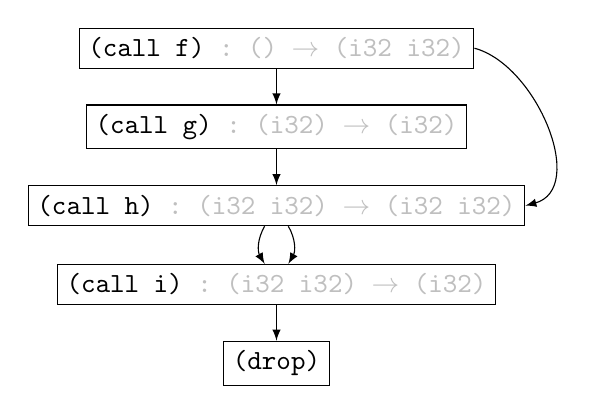
\begin{tikzpicture}
    \node[draw] (f) at (0, 0) {\texttt{(call f)\color{lightgray}~:~() $\to$ (i32 i32)}};
    \node[draw] (g) at (0, -1) {\texttt{(call g)\color{lightgray}~:~(i32) $\to$ (i32)}};
    \node[draw] (h) at (0, -2) {\texttt{(call h)\color{lightgray}~:~(i32 i32) $\to$ (i32 i32)}};
    \node[draw] (i) at (0, -3) {\texttt{(call i)\color{lightgray}~:~(i32 i32) $\to$ (i32)}};
    \node[draw] (d) at (0, -4) {\texttt{(drop)}};

    \draw[->,>=latex] (f) to (g);
    \draw[->,>=latex] (f.east) to[in=15, out=-15] (h.east);
    \draw[->,>=latex] (g) to (h);
    \draw[->,>=latex] (h) to[bend right] (i);
    \draw[->,>=latex] (h) to[bend left] (i);
    \draw[->,>=latex] (i) to (d);
  \end{tikzpicture}
  \caption{Non classical data flow with multiple return values}\label{data-flow}
\end{figure}

\textsf{Watib}'s IR is closer to modern Wasm. We represent the instructions in a
linear way. It allows to output code that use block parameters without
additional burden for instance. We hope that will enable different optimisations
and a better treatment of code written using WebAssembly's new features.

\section{Validation}\label{val}
We start by giving an overview of WebAssembly's type system, and then describe
our implementation of it.
\subsection{WebAssembly's type system}

WebAssembly's type system supports \emph{declared and mutually iso-recursive
subtyping}.
Wasm's subtyping is \emph{declared} as the subtyping relations between the
defined types have to be specified as part of the type defintion. Their validity
can be checked with the type definition's validation.

We now give the intuition behind \emph{mutually iso-recursive subtyping} ---
see~\cite{rossberg2023mutually} for a full discussion.
\subsection{A type checker for WebAssembly}
The typing rules given by the third section of the specification are purely
declarative. They give more than one type to many instructions and rely on the
transitivity rule of subtyping, which can't be implemented as is. If we want to
check that $t_1 \leq t_2$ in presence of transitivity, we need to choose a third
type to compare it to $t_1$ and $t_2$, which complicates subtyping. We, thus,
needed to adapt them to implement a type checker. Our type-checker is similar to
the one shipped we the specification. For the subtyping of \emph{value types},
we rewrote the rules to have equivalent ones without the transitivity
rules\footnote{they are implemented by the function \texttt{<ht=} of the
\texttt{Type/match.scm} and reproduced in Appendix~\ref{subtyping}} and for
\emph{instruction types}, we rely on a stack and most general types, as
explained in the next paragraph.

To check a sequence of instructions we maintain an internal state recording the
types of the elements present on the stack, instead of analysing each
instruction individually and checking that the types compose well --- which is
what is described by the declarative rules.

Most instructions have a most general type (i.e. a type subtype of all the other
types we can type the instruction with) or are not exited (like unconditional
branches). The typing rules for the latter are $i:{t_1}^*t^*\to {t_2}^*$ for all
$t_1$ and $t_2$. We represent it as ${t_1}^*t^*\to {t_2}^*$, where \textsf{poly}
is a special symbol indicating that the stack can be whatever we need it to be
--- it can be thought as a type variable, on which we do not perform explicit
unification. When we refer to the type one of those instruction, we mean its
most general type or the type with the \textsf{poly} symbol, these types are
contined in the file \texttt{Val/instruction-types.sch}. The instructions that
do not fall in either category (for instance, \textsf{ref.as\_non\_null} has
type $\refnullt ht\to \reft ht$ for all heap type $ht$) are treated in a
separate function, they peek on the stack to compute their output type, avoiding
the use of type variables.

We describe how one instruction $i$ modifies the state of this stack. Either the
instruction is treated in an ad-hoc way

\begin{itemize}
\item Let ${t_1}^*\to{t_2}^*$ be the type of $i$.
\end{itemize}
\section{Optimisation}\label{opt}
\textsf{Watib} performs several optimisation passes. They all take care to
maintain typing information. As we show it later, some code is unnecessary
execution-wise but needs to be kept to maintain well-typedness.

We start by reviewing optimisations which benefit the others, by giving more
precise information or removing generated useless code.

\begin{description}
  \item[Copy Propagation] When a variable $x$ is assigned the value of another
    variable $y$, we replace references to $x$ with references to $y$, until the
    next assignement to $x$ or $y$. We were inspired
    by~\cite[Section~12.5]{muchnick1997advanced} approach.
  \item[Pure Drops Elimination] We eliminate \textsf{drop} instructions and
    their argument when it has no side effect. We try to remove as extra
    computation as possible by inserting as much \textsf{drop} as needed.
  \item[Constant Folding] We evaluate some expressions whose value is known at
    compile time. We also also remove conditional branching when the condition
    is constant.
  \item[Unreachable Code Elimination] We eliminate some instructions that are
    known to never execute (after a \textsf{return} for instance). However, some
    dead code may be needed for validation, even though it can't be executed.
    For instance, removing the \textsf{(unreachable)} instruction at the end of
    the function of Figure~\ref{ex} makes it ill-typed. The \textsf{if}
    instruction puts nothing on the stack while the function expects an
    \textsf{i32} on top of the stack. When well-typedness without the dead
    instructions can't easily be guaranteed, an \textsf{unreachable} instruction
    is inserted instead of the dead code.
  \item[Peephole optimisation] We recognise small patterns in Wasm code and
    replace them with equivalent code that is smaller or faster.
  \item[Type propagation] This one is not an optimisation \emph{per se}. It only
    refines type annotations of variables in the IR. When a variable is assigned
    a value, the type of this value (which may be a strict subtype of the
    variable's declared type) is set as the actual output type of each variable
    access, until it is modified.
\end{description}

Most optimisations passes described earlier are general, in the sense that they
are applied in most optimising compilers~\cite{muchnick1997advanced}. We, now,
review more Wasm-specific optimisations and detail in which way they use the
previous ones.
\subsection{Cast Elimination}
We eliminate redundant casts and replace type tests by constants if their result
can be determined. Such casts and tests could be introduced by copy-propagation
as when we may replace a variable with another one of a smaller type or by the
next optimisation. To stay conservative about side-effects eliminated tests are
replaced by a \textsf{(drop)} and the result of the test, which is a constant.
Pure Drop Elimination will remove some useless computation. Constant folding
will propagate the result of the test.

To check for type tests to eliminate, we compare the argument's actual type
(which may be smaller than its static type) against the type it is tested for.
For casts, we only check against the static type as the cast can be necessary to
maintain well-typedness.

\subsection{Type-Dependent Control Flow Rewriting}\label{broncast}
A common pattern in the Wasm code generated by the Bigloo compiler is a
branching on a type test, and the use of casts in case the test is successful,
like in Figure~\ref{ex}. If Wasm wasn't statically typed, these casts could be
removed by an optimising compiler that would determine that they are redundant.

\subsection{Control-Flow Graph transformation}
\section{Benchmarks}\label{bench}
\section{Conclusion}
\printbibliography
\newpage
\appendix
\section{Wasm-as' extensions to the specification}\label{wasmasex}
\section{Matching rules for \emph{heap types}}\label{subtyping}
\begin{mathpar}
  \inferrule{t_1 = t_2}{C\vdash t_1\leq t_2}\hfill
  \inferrule{\\}{C\vdash \bot\leq t}\hfill
  \inferrule{C\vdash C.\text{\textsf{types}}[x]\leq t}{C\vdash x \leq t}\hfill
  \inferrule{C\vdash t \leq C.\text{\textsf{types}}[x]}{C\vdash t \leq x}\\
  \inferrule{C\vdash t\leq\text{\textsf{any}}}
            {C\vdash\text{\textsf{none}}\leq t}\hfill
  \inferrule{C\vdash t\leq\text{\textsf{func}}}
            {C\vdash\text{\textsf{nofunc}}\leq t}\hfill
  \inferrule{C\vdash t\leq\text{\textsf{extern}}}
            {C\vdash\text{\textsf{noextern}}\leq t}\hfill
  \inferrule{C\vdash t\leq\text{\textsf{exn}}}
            {C\vdash\text{\textsf{noexn}}\leq t}\\
  \inferrule{C\vdash t\leq\text{\textsf{any}}}
            {C\vdash t\leq\text{\textsf{eq}}}\hfill
  \inferrule{\\}{C\vdash\text{\textsf{i31}}\leq\text{\textsf{eq}}}\hfill
  \inferrule{\\}{C\vdash\text{\textsf{struct}}\leq\text{\textsf{eq}}}\hfill
  \inferrule{\\}{C\vdash\text{\textsf{array}}\leq\text{\textsf{eq}}}\\
  \inferrule{\text{\textsf{unroll}} (deftype)= (symbol\ldots)}
            {C\vdash deftype\leq\text{\textsf{symbol}}}\hfill
\inferrule{\text{\textsf{unroll}} (deftype)= (symbol\ldots)\\ C\vdash symbol\leq\text{\textsf{eq}}}
            {C\vdash deftype\leq\text{\textsf{eq}}}
\end{mathpar}
\end{document}
